\documentclass{../notes}

\title{DM n°2 -- \itshape Logique}
\author{Hugo \scshape Salou}

\newcommand\zf[1]{\hyperref[ZF#1]{\textsf{ZF\,#1}}}
\newcommand\fond{\hyperref[FOND]{\textsf{Fond}}}
\newcommand\inphi[1][\relax]{\ensuremath{\mathrel{\varepsilon_{\varphi_{#1}}}}}

\newcommand\head{\setmainfont{Noto Emoji}[FontFace = {sb}{n}{ Font={*}, FakeBold = 1.2 }]\fontseries{sb}\selectfont \makebox[5pt][c]{😈}}
\newcommand\sword{\setmainfont{Noto Emoji}[FontFace = {sb}{n}{ Font={*}, FakeBold = 1.2 }]\fontseries{sb}\selectfont \makebox[5pt][c]{\rotatebox{-45}{⚔️}}}


\begin{document}
  \maketitle

  \chapter{Parties finies de $\mathds{N}$.}

  \begin{enumerate}
    \item Montrons que l'univers $\langle \mathds{N}, {\inphi} \rangle$ satisfait \zf 1, \zf 2, \zf 3 et \zf 4.
      \begin{description}
        \item[ZF\,1.] \label{ZF1}
          $\forall x\: \forall y\: (\forall z \: (z \in x \leftrightarrow z \in y) \leftrightarrow x = y)$.

          Soient $x, y \in \mathds{N}$. On a la chaîne d'équivalences :
          \begin{align*}
            \hspace{-5em}
            x = y & \text{ ssi } \varphi(x) = \varphi(y) && \text{ car $\varphi$ injective }\\
                  & \text{ ssi } \forall z \in \mathds{N}, z \in \varphi(x) \iff z \in \varphi(y) && \text{ par égalité d'ensembles }\\
                  & \text{ ssi } \forall z \in \mathds{N}, z \inphi x \iff z \inphi y && \text{ par définition}
          .\end{align*}
          D'où \zf 1 est vérifié par l'univers $\langle \mathds{N}, \inphi \rangle$.

        \item[ZF\,2.] \label{ZF2} $\forall  x \: \exists  y \: \forall  t \: t \in y \leftrightarrow \exists  z \: (t \in z \land z \in x)$.

          Soit $x \in \mathds{N}$. L'ensemble $\bigcup_{z \in \varphi(x)} \varphi(z)$ est une union finie (car $\varphi(x)$ fini) de parties finies de $\mathds{N}$ (car les $\varphi(z)$ sont finies).
          Par surjectivité de $\varphi$, il existe un entier $y \in \mathds{N}$ tel que $\varphi(y) = \bigcup_{z \in \varphi(x)} \varphi(z)$.
          Soit $z \in \mathds{N}$. On a la chaîne d'équivalences suivante :
          \begin{align*}
            \hspace{-5em}
            t \inphi y & \text{ ssi } t \in \varphi(y) && \text{ par définition de $\inphi$ }\\
                       & \text{ ssi } t \in \bigcup_{z \in \varphi(x)} \varphi(z) && \text{ par définition de $y$ }\\
                       & \text{ ssi } \exists z \in \varphi(x), t \in \varphi(z) && \text{ par union ensembliste }\\
                       & \text{ ssi } \exists z \in \mathds{N} \: z \inphi x \text{ et } t \inphi z && \text{ par définition}
          .\end{align*}
          D'où \zf 2 est vérifié par l'univers $\langle \mathds{N}, \inphi \rangle$.

        \item[ZF\,3.] \label{ZF3}
          $\forall  a \: \exists b \: t \in b \leftrightarrow \overbrace{\forall z (z \in t \to z \in a)}^{\textstyle t \subseteq a}$.

          Soit $a \in \mathds{N}$.
          L'ensemble $\wp(\varphi(a))$ des parties de $\varphi(a)$ est fini (de cardinal $2^{\# \varphi(a)}$).
          Comme $\varphi$ surjective, on a $\wp(\varphi(a)) = \{\varphi(k)  \mid  \varphi(k) \subseteq \varphi(a)\}$.
          Ainsi, par image réciproque de cet ensemble par l'isomorphisme $\varphi$, on a que l'ensemble $B := \{k \in \mathds{N}  \mid  \varphi(k) \subseteq \varphi(a)\}$ est une partie finie de $\mathds{N}$ (même cardinal).
          Comme $\varphi$ surjective, il existe un entier $b \in \mathds{N}$ tel que $\varphi(b) = B$.
          On a la chaîne d'équivalences suivante :
          \begin{align*}
            \hspace{-5em}
            t \inphi b & \text{ ssi } t \in \varphi(b) = B && \text{ par définition de $\inphi$ et $b$ }\\
                       & \text{ ssi } \varphi(t) \subseteq \varphi(a) && \text{ par définition de $B$ }\\
                       & \text{ ssi } \forall  z \in \mathds{N}, z \in \varphi(t) \implies z \in \varphi(a) && \text{ par définition de $\subseteq$ }\\
                       & \text{ ssi } \forall z \in \mathds{N}, z \inphi t \implies z \inphi a && \text{ par définition}
          .\end{align*}
          D'où \zf 3 est vérifié par l'univers $\langle \mathds{N}, \inphi \rangle$.

        \item[ZF\,4.] \label{ZF4}
          Pour toute formule $\psi$ à $n+2$ paramètres, 
          \[
            \scriptstyle
            \forall v_1 \; \ldots \; \forall v_n \; \mathrm{fonc}_\psi (v_1, \ldots, v_n) \to \forall u \; \exists v \; \forall w \; 
          (w \in u \leftrightarrow \exists x \; x \in u \land \psi(x, w, v_1, \ldots, v_n))
          \]
          où $ \scriptstyle \mathrm{fonc}_\psi(v_1, \ldots, v_m) := \forall x \, \forall y_1 \, \forall y_2 \; \psi(x, y_1, v_1, \ldots, v_n) \land \psi(x, y_2, v_1, \ldots, v_n) \to y_1 = y_2$.

          Soit $\psi$ une formule à $n+2$ paramètres.
          Soient $v_1, \ldots, v_n$ et supposons $\psi$ fonctionnelle en son premier paramètre.
          Soit $u \in \mathds{N}$.
          De par cette hypothèse de relation fonctionnelle, pour tout $x \in \varphi(u)$, il existe au plus un entier $w$ tel que $\varphi(x, w, v_1, \ldots, v_n)$ soit vraie.
          Ainsi l'ensemble \[
            V := \mleft\{\,w \in \mathds{N} \;\middle|\; \exists x \in \varphi(u), \psi(x, w, v_1, \ldots, v_n) \text{ vraie}\,\mright\} 
          \] est fini (car cardinal majoré par $\#\varphi(u)$, fini).
          Il existe donc un entier $v \in \mathds{N}$ tel que $\varphi(v) = V$ (par surjectivité de $\varphi$).
          Soit $w \in \mathds{N}$.
          On a la chaîne d'équivalences suivante :
          \begin{align*}
            \hspace{-7em}
            w \inphi v & \text{ ssi } w \in \varphi(v) = V && \text{ par déf. de $\inphi$ et $v$ }\\
                       & \text{ ssi } \exists x \in \varphi(u), \psi(x, w, v_1, \ldots, v_n) \text{ vraie } && \text{ par déf. de $V$ }\\
                       & \text{ ssi } \exists x \in \mathds{N}, x \inphi u \text{ et } \psi(x, w, v_1, \ldots, v_n) &&\text{ par déf. de $\inphi$}
          .\end{align*}
          D'où \zf 4 est vérifié par l'univers $\langle \mathds{N}, \inphi \rangle$.
      \end{description}
    \item \label{ex1q2} Supposons que, pour tous $x, y \in \mathds{N}$, $x \in \varphi(n)$ implique $x < y$.
      Montrons que $\langle \mathds{N}, {\inphi}\rangle$ vérifie \fond.
      \begin{description}
        \item[Fond.]\label{FOND}
          $\forall x \: x \neq \emptyset \to \exists y \: y \in x \land x \cap y = \emptyset$\\
          où l'on note\footnote{Ces notations sont précisées uniquement pour expliciter comment "placer" $\inphi$ dans une intersection ou une égalité d'ensemble. On utilise implicitement l'axiome d'extensionnalité \zf 1}\showfootnote :
          \begin{itemize}
            \item $x \neq \emptyset$ pour $\exists v \: v \in x$
            \item $x \cap y = \emptyset$ pour $\forall w \: \lnot (w \in x \land w \in y)$
          \end{itemize}

      \end{description}

      Soit $x \in \mathds{N}$ et supposons qu'il existe $v$ tel que $v \inphi x$, on a donc~$\varphi(x) \neq \emptyset$.
      La partie non-vide $\varphi(x)$ admet ainsi un minimum que l'on note $y \in \varphi(x)$.
      On a bien $y \inphi x$ par minimum.
      De plus, soit  $w \in \mathds{N}$ et supposons (par l'absurde) $w \inphi x$ et $w \inphi y$.
      Alors $w \in \varphi(y)$ et donc  $w < y$ par hypothèse.
      Or, $w \in \varphi(x)$. Absurde car $y$ est le minimum de $\varphi(x)$.

      D'où, avec l'implication "$\inphi$ implique $<$", l'univers $\langle \mathds{N}, \inphi \rangle$ vérifie \fond.
    \item
      Pour un entier $n \in \mathds{N}$, on note $\mathsf{bin}(n)_i \in \{\mathtt{0}, \mathtt{1}\} $ le $i$-ème bit dans l'écriture binaire de $n$.
      La fonction $\mathsf{bin}$ donne une bijection entre $\mathds{N}$ et l'ensemble des suite de $\{\mathtt{0}, \mathtt{1}\}$ n'ayant qu'un nombre fini de $\mathtt{1}$.
      En effet, l'écriture binaire d'un entier est unique et n'utilise qu'un nombre fini de $\mathtt{1}$.
      Réciproquement, on peut interpréter une suite de $\{\mathtt{0}, \mathtt{1}\}$ n'ayant qu'un nombre fini de $\mathtt{1}$ (correspondant aux indices $i_1 < i_2 < \cdots < i_n$) en un entier $\sum_{k = 1}^n 2^{i_k} < \infty$.

      Considérons ainsi la bijection :
      \begin{align*}
        \varphi_1: \mathds{N} &\longrightarrow \mathsf{W} \\
        n &\longmapsto \mleft\{\, i \;\middle|\; \mathsf{bin}(n)_i = \mathtt{1}\,\mright\} 
      .\end{align*}
      C'est en effet une bijection car :
      \begin{itemize}
        \item (injectivité) un entier est défini de manière unique par son écriture binaire (on donne les positions des $\mathtt{1}$, on en déduit l'écriture binaire en mettant des $\mathtt{0}$ ailleurs, et bijection $\mathsf{bin}$ précédente) ;
        \item (surjectivité) pour tout partie $A \in \mathsf{W}$, on considère l'entier $\sum_{a \in A} 2^a < \infty$ qui vérifie $\varphi_1(a) = A$.
      \end{itemize}

      L'univers $\langle \mathds{N}, \inphi[1] \rangle$ vérifie \fond\ car, d'après la question~\ref{ex1q2}, il suffit que "$\inphi[1]$ implique  $<$".
      Supposons $x \in \varphi_1(y)$, où $x, y \in \mathds{N}$.
      D'où, $\mathsf{bin}(y)_x = \mathtt{1}$ par définition de $\varphi_1$, et donc $y \ge 2^x > x$.

      Considérons ensuite la fonction $\mathsf{swap} : \mathds{N}\to \mathds{N}$ qui échange les deux derniers bits dans l'écriture binaire d'un entier.
      C'est bien une bijection (c'est son propre inverse).

      On pose la bijection $\varphi_2 := \varphi_1 \circ \mathsf{swap}$ (composée de deux bijections).
      L'univers $\langle \mathds{N}, \inphi[2] \rangle$ ne vérifie pas \fond.
      En effet, d'après le TD n°11, on a que $\fond, \zf 1, \zf 2, \zf 3, \zf 4 \vdash \forall x \: \lnot (x \in x)$ (on n'a pas utilisé \zf 5 dans la preuve).
      Or, on a \[
        \varphi_2(1) = \varphi_2(\overbrace{\overline{\mathtt{\cdots001}}}^1) = \varphi_1(\overbrace{\overline{\mathtt{\cdots 010}}}^2) = \{1\} 
      ,\]
      et donc $1 \inphi[2] 1$.
  \end{enumerate}

  \chapter{Hydre de Lerne.}

  \begin{enumerate}
    \item Afin de simplifier les calculs, on remarque que :
      \begin{itemize}
        \item $\displaystyle f\left(
            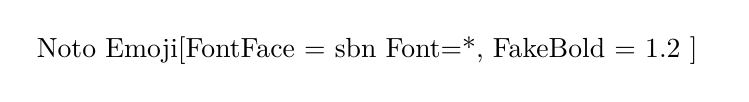
\begin{tikzpicture}[baseline=-1mm,scale=0.6, sibling distance=15mm]
              \node { \head };
            \end{tikzpicture}
          \right) = 0$ ;
        \item $\displaystyle f\left(
            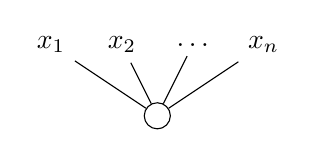
\begin{tikzpicture}[baseline={(current bounding box.center)},scale=0.6, sibling distance=15mm]
              \node[draw, circle] {} [grow'=up]
              child {node {$x_1$}}
              child {node {$x_2$}}
              child {node {$\ldots$}}
              child {node {$x_n$}}
              ;
            \end{tikzpicture}
          \right) = \sum_{i=1}^n \omega^{f(x_i)}$ 
      \end{itemize}
      où la somme se fait dans l'ordre croissant (càd, de la branche la plus lourde à la plus légère).

      Pour la première hydre, on a :
      \[
        f \left(
            \begin{tikzpicture}[baseline={(current bounding box.center)},scale=0.6, sibling distance=15mm]
              \node[draw,circle,fill=deepgreen] {} [grow'=up]
                child {node {\head}}
                child {node[draw, circle] {}
                  child { node {\head} }
                  child { node {\head} }
                  child { node {}
                    node[draw, circle] {}
                     child { node {\head} }
                  }
                }
              ;
            \end{tikzpicture}
          \right)
          = \omega^{\omega^{\omega^0} + \omega^0 + \omega^0} + \omega^0 = \omega^{\omega + 2} + 1
      .\] 

      Pour la deuxième, on a 
      \[
        f \left(
            \begin{tikzpicture}[baseline={(current bounding box.center)},scale=0.6, sibling distance=15mm]
              \node[draw,circle,fill=deepgreen] {} [grow'=up]
                child {node {\head}}
                child {node[draw, circle] {}
                  child { node {\head} }
                  child { node {\head} }
                  child { node {\head} }
                  child { node {\head} }
                }
              ;
            \end{tikzpicture}
          \right)
          = \omega^{\omega^0 + \omega^0 + \omega^0 + \omega^0} + \omega^0 = \omega^{4} + 1
      .\] 

      Pour la troisième, on a 
      \[
        f \left(
            \begin{tikzpicture}[baseline={(current bounding box.center)},scale=0.6, sibling distance=15mm]
              \node[draw,circle,fill=deepgreen] {} [grow'=up, sibling distance=30mm]
                child {node {\head}}
                child {node[draw, circle] {} [sibling distance=10mm]
                  child { node {\head} }
                  child { node {\head} }
                  child { node {\head} }
                }
                child {node[draw, circle] {} [sibling distance=10mm]
                  child { node {\head} }
                  child { node {\head} }
                  child { node {\head} }
                }
                child {node[draw, circle] {} [sibling distance=10mm]
                  child { node {\head} }
                  child { node {\head} }
                  child { node {\head} }
                }
              ;
            \end{tikzpicture}
          \right)
          = \omega^3 \cdot 3 + 1
      .\]
      On remarque que, dans notre exemple, chaque valeur de l'hydre décroît strictement après un coup.
    \item On part de $H_0$ et on construit $\alpha_0$ la valeur de l'hydre $H_0$ donnée sous forme normale de Cantor.
      En effet, en calculant $f(r)$ à l'aide de la définition inductive précédente de $f$, où  $r$ est la racine de l'hydre $H_0$, on obtient directement un ordinal sous forme normale de Cantor (il suffit de regrouper les $\omega^{f(x_i)}$ identiques dans la somme).

      Étudions le cas du $i$-ème coup de Héraclès, et son effet sur la valeur de l'hydre (càd. le changement $H_i \leadsto H_{i+1}$).
      Localement, la situation est la suivante.

      \begin{adjustbox}{center}
        \begin{tikzpicture}[baseline={(current bounding box.center)},scale=0.6, sibling distance=15mm]
          \node[draw,circle] {\clap{1}} [grow'=up, sibling distance=30mm]
            child [dashed] {node[dashed,draw,rectangle] {$\mathit{avant}$}}
            child {node[draw,circle] (r) {\clap{2}}
              child [dashed] {node[dashed,draw,rectangle] {$\mathit{autres}$}}
              child {node (h) {\head}}
            }
            child [dashed] {node[dashed,draw,rectangle] {$\mathit{après}$}}
          ;
          \draw (r) to node[midway,nicered] {\sword} (h);
        \end{tikzpicture}
      \end{adjustbox}

      \begin{adjustbox}{center}
        {\LARGE $ \vertical\leadsto $}
      \end{adjustbox}

      \begin{adjustbox}{center}
        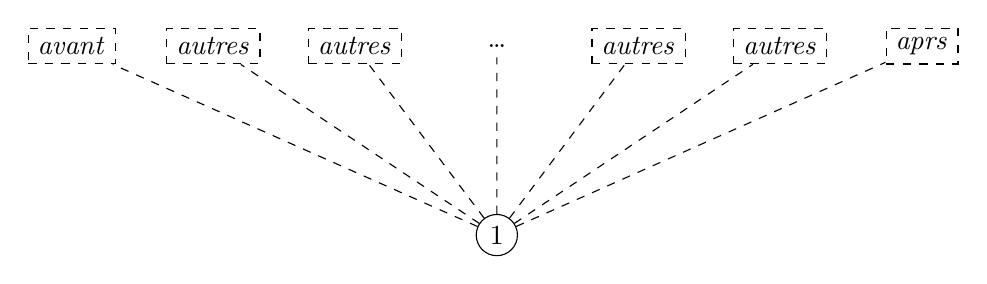
\begin{tikzpicture}[baseline={(current bounding box.center)},scale=0.6, sibling distance=15mm]
          \node[draw,circle] {\clap{1}} [grow'=up, sibling distance=3cm, level distance=4cm]
            child [dashed] {node[dashed,draw,rectangle] {$\mathit{avant}$}}
            child [dashed] {node[dashed,draw,rectangle] {$\mathit{autres}$}}
            child [dashed] {node[dashed,draw,rectangle] {$\mathit{autres}$}}
            child [dashed] {node {\ldots}}
            child [dashed] {node[dashed,draw,rectangle] {$\mathit{autres}$}}
            child [dashed] {node[dashed,draw,rectangle] {$\mathit{autres}$}}
            child [dashed] {node[dashed,draw,rectangle] {$\mathit{après}$}}
          ;
        \end{tikzpicture}
      \end{adjustbox}

      On coupe la tête et on crée $i$ copies du "groupe" $\mathit{autres}$.
      Les tracés en pointillés indiquent qu'il y a potentiellement plusieurs arêtes/nœuds (voire aucun).

      La valeur de la "sous-hydre locale" est initialement (sous forme normale de Cantor) \[
      \alpha = \omega^{\beta_1} \cdot n_1 + \cdots + \omega^{\beta_k} \cdot n_k
      .\]
      Comme on coupe une tête, correspondant à l'une des arêtes, on change l'un des termes en haut, et uniquement un seul (en effet, sinon, on changerait deux branches de poids différents).
      Nommons $\ell \in \llbracket 1, k\rrbracket$ l'indice du terme $\omega^{\beta_\ell} \cdot n_\ell$ changé.
      Soit $\omega^{\gamma} \cdot m$ le terme modifié.
      Montrons \[
        \hspace{-4.5em}
        \sum_{i=1}^{\ell-1} \omega^{\beta_i} n_i 
        +
        \omega^{\beta_\ell} (n_\ell - 1) + 
        \omega^{\beta_\ell}
        +
        \sum_{i=\ell+1}^{k} \omega^{\beta_i} n_i > 
        \sum_{i=1}^{\ell-1} \omega^{\beta_i} n_i 
        +
        \omega^{\beta_\ell} (n_\ell - 1) + 
        \omega^{\gamma} m
        +
        \sum_{i=\ell+1}^{k} \omega^{\beta_i} n_i
      .\]
      Pour cela, il suffit (TD n°11) de montrer que \[
        \omega^{\beta_\ell}
        +
        \sum_{i=\ell+1}^{k} \omega^{\beta_i} n_i > 
        \omega^{\gamma} m
        +
        \sum_{i=\ell+1}^{k} \omega^{\beta_i} n_i
        \quad (\star)
      .\]

      On applique le lemme suivant.

      \textbf{Lemme.}
      \begin{slshape}
        Pour tous ordinaux $\beta > \beta'$ et $k \in \omega$, on a $\omega^{\beta} > \omega^{\beta'} \cdot k$.
      \end{slshape}

      \textit{Preuve.} Par induction transfinie sur $\beta$, on a trois cas.
      \begin{itemize}
        \item Pour $\beta = 0$, c'est vrai par vacuité.
        \item Pour $\beta + 1$, en supposant la propriété vraie pour $\beta$, soit $\beta' < \beta + 1$.
          On a deux cas :
           \begin{itemize}
            \item \textit{\textbf{Cas 1.}} Si $\beta' = \beta$ alors, on a $\omega > k$ et donc \[
              \omega^{\beta+1} = \omega^{\beta}\omega > \omega^{\beta}k
              .\] 
            \item \textit{\textbf{Cas 2.}} Si $\beta' < \beta$ alors on applique l'hypothèse de récurrence pour $\beta$ et on a le résultat.
          \end{itemize}
        \item Pour $\bigcup_{\gamma < \beta} \gamma$, en supposant la propriété vraie pour tout $\gamma < \beta$, soit $\beta' < \bigcup_{\gamma < \beta} \gamma$.
          Ainsi, il existe $\delta$ tel que $\beta' < \delta < \beta$.
          De plus, $\delta > 0$ car $0 \le \beta' < \delta$.
          On a donc :
          \[
            \omega^{\bigcup_{\gamma < \beta} \gamma} \underset{\text{(déf.)}}= \bigcup_{0 < \gamma < \beta} \omega^{\gamma} \underset{\text{(sup.)}}\ge \omega^{\delta} \underset{\text{(I.H.)}}> \omega^{\beta'} \cdot k
          .\]
      \end{itemize}
      On conclut par induction transfinie. \hfill $\square$

      Ainsi, on a que $\omega^{\beta_\ell} > \omega^{\gamma} m$ par le lemme précédent.
      On a donc \[
      \omega^{\beta_\ell} + \sum_{i=\ell+1}^k \omega^{\beta_i} n_i \ge \omega^{\gamma} m + \sum_{i=\ell+1}^k \omega^{\beta_i} n_i
      .\]
      Pour éliminer le cas de l'égalité, il suffit de remarquer que, si ces deux termes étaient égaux, alors par unicité de la forme normale de Cantor, on aurait $\beta_\ell = \gamma$, absurde !

      Ceci permet de conclure que, localement, la valeur de l'hydre décroit strictement.

      Pour conclure sur la valeur de l'arbre, on montre que la stricte décroissance de la valeur est préservée en remontant dans l'arbre.
      Le cas initial est déjà fait.
      Dans l'hérédité, la situation est la suivante :

      \begin{adjustbox}{center}
        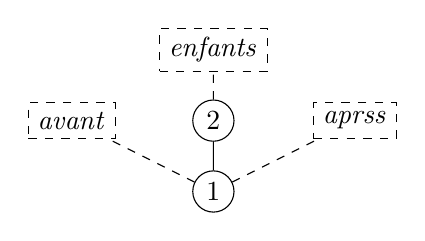
\begin{tikzpicture}[baseline={(current bounding box.center)},scale=0.6, sibling distance=15mm]
          \node[draw,circle] {\clap{1}} [grow'=up, sibling distance=30mm]
            child [dashed] {node[dashed,draw,rectangle] {$\mathit{avant}$}}
            child {node[draw,circle] {\clap{2}}
              child [dashed] {node[dashed,draw,rectangle] {$\mathit{enfants}$}}
            }
            child [dashed] {node[dashed,draw,rectangle] {$\mathit{aprèss}$}}
          ;
        \end{tikzpicture}
      \end{adjustbox}

      \begin{adjustbox}{center}
        {\LARGE $ \vertical\leadsto $}
      \end{adjustbox}

      \begin{adjustbox}{center}
        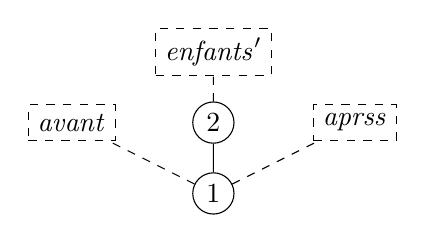
\begin{tikzpicture}[baseline={(current bounding box.center)},scale=0.6, sibling distance=15mm]
          \node[draw,circle] {\clap{1}} [grow'=up, sibling distance=30mm]
            child [dashed] {node[dashed,draw,rectangle] {$\mathit{avant}$}}
            child {node[draw,circle] {\clap{2}}
              child [dashed] {node[dashed,draw,rectangle] {$\mathit{enfants}'$}}
            }
            child [dashed] {node[dashed,draw,rectangle] {$\mathit{aprèss}$}}
          ;
        \end{tikzpicture}
      \end{adjustbox}
      
      où $\mathit{enfants} \leadsto \mathit{enfants}'$.

      La valeur passe donc de \[
        \sum_{i=1}^{\ell - 1} \omega^{\beta_i} n_i + 
        \omega^{\beta_\ell} (n_\ell - 1) +
        \omega^{\beta_\ell} +
        \sum_{i=\ell+1}^n \omega^{\beta_i} n_i
      \]
      à \[
        \sum_{i=1}^{\ell - 1} \omega^{\beta_i} n_i + 
        \omega^{\beta_\ell} (n_\ell - 1) +
        \omega^{\gamma} +
        \sum_{i=\ell+1}^n \omega^{\beta_i} n_i
      .\]

      Ce cas est identique au précédent (avec $m = 1$).
      On a donc bien la décroissance stricte à cette étape.

      On en conclut que, à chaque coup, la valeur de l'hydre décroit strictement.
      Or, l'ordre $<$ est bien fondé sur les ordinaux donc, au bout d'un nombre fini de coups, la valeur de l'hydre arrive à une valeur de $0$ : Héraclès a battu l'hydre de Lerne.
  \end{enumerate}

  \begin{slshape}
    Cet exercice peut être réalisé beaucoup plus simplement avec le lemme de König ou, mieux encore, l'extension multiensemble (\textit{c.f.} cours de Th.Prog.).
    En effet, considérons le multiensemble des profondeurs des têtes.
    Après le $i$-ème coup, on retire une tête de profondeur $d$ et on en fait apparaître $i$ à la profondeur $d - 1$, d'où cette suite de multiensembles décroit strictement pour $>_\mathrm{mul}$.
    Or, en Th.Prog., on a vu que $>_\mathrm{mul}$ est terminante ssi $>_\mathds{N}$ est terminante, et on sait que la relation $>_\mathds{N}$ est terminante.
    Ceci donne une preuve alternative, beaucoup plus simple, et qui n'utilise pas les ordinaux.
  \end{slshape}


  \vfill

  \begin{center}
    \color{deepblue}
    \bfseries
    \itshape
    --- Fin du DM ---
  \end{center}

  \vfill
\end{document}
